%%
\chapter{SquatGAN: Architettura e Design}

\section{Architettura}
Il sistema SquatGAN è basato quindi sull'utilizzo principale di una rete neurale generativa convoluzionale (DCGAN), la cui struttura verrà spiegata nei capitoli successivi, e a supporto della rete neurale sono stati aggiunti moduli di supporto, ognuno dei quali con una funzionalità specifica.\\
Ciò che segue è una spiegazione ad alto livello dell'architettura di SquatGAN in cui verranno illustrati i vari componenti che sono stati necessari alla realizzazione di quest'ultimo.\\
Come mostrato in figura \ref{fig:arch1}, il primo modulo implementato mi permette di produrre un dataset di immagini che sono necessarie per l'addestramento della rete neurale. In secondo luogo abbiamo la rete generativa convoluzionale che riceve come input il dataset di immagini generate e che utilizzerà per addestrare la rete nell'apprendimento e la generazione di nuove immagini. Infine ho implementato un modulo per il riconoscimento ottico di caratteri (OCR. Optical Character Recognition) in modo che le immagini generate dalla rete neurale potessero essere interpretate e tradotte in stringhe di testo (che alla fine saranno i domini di squatting generati).
\begin{figure}[!h]
  \centering
  \begin{minipage}[b]{0.6\textwidth}
    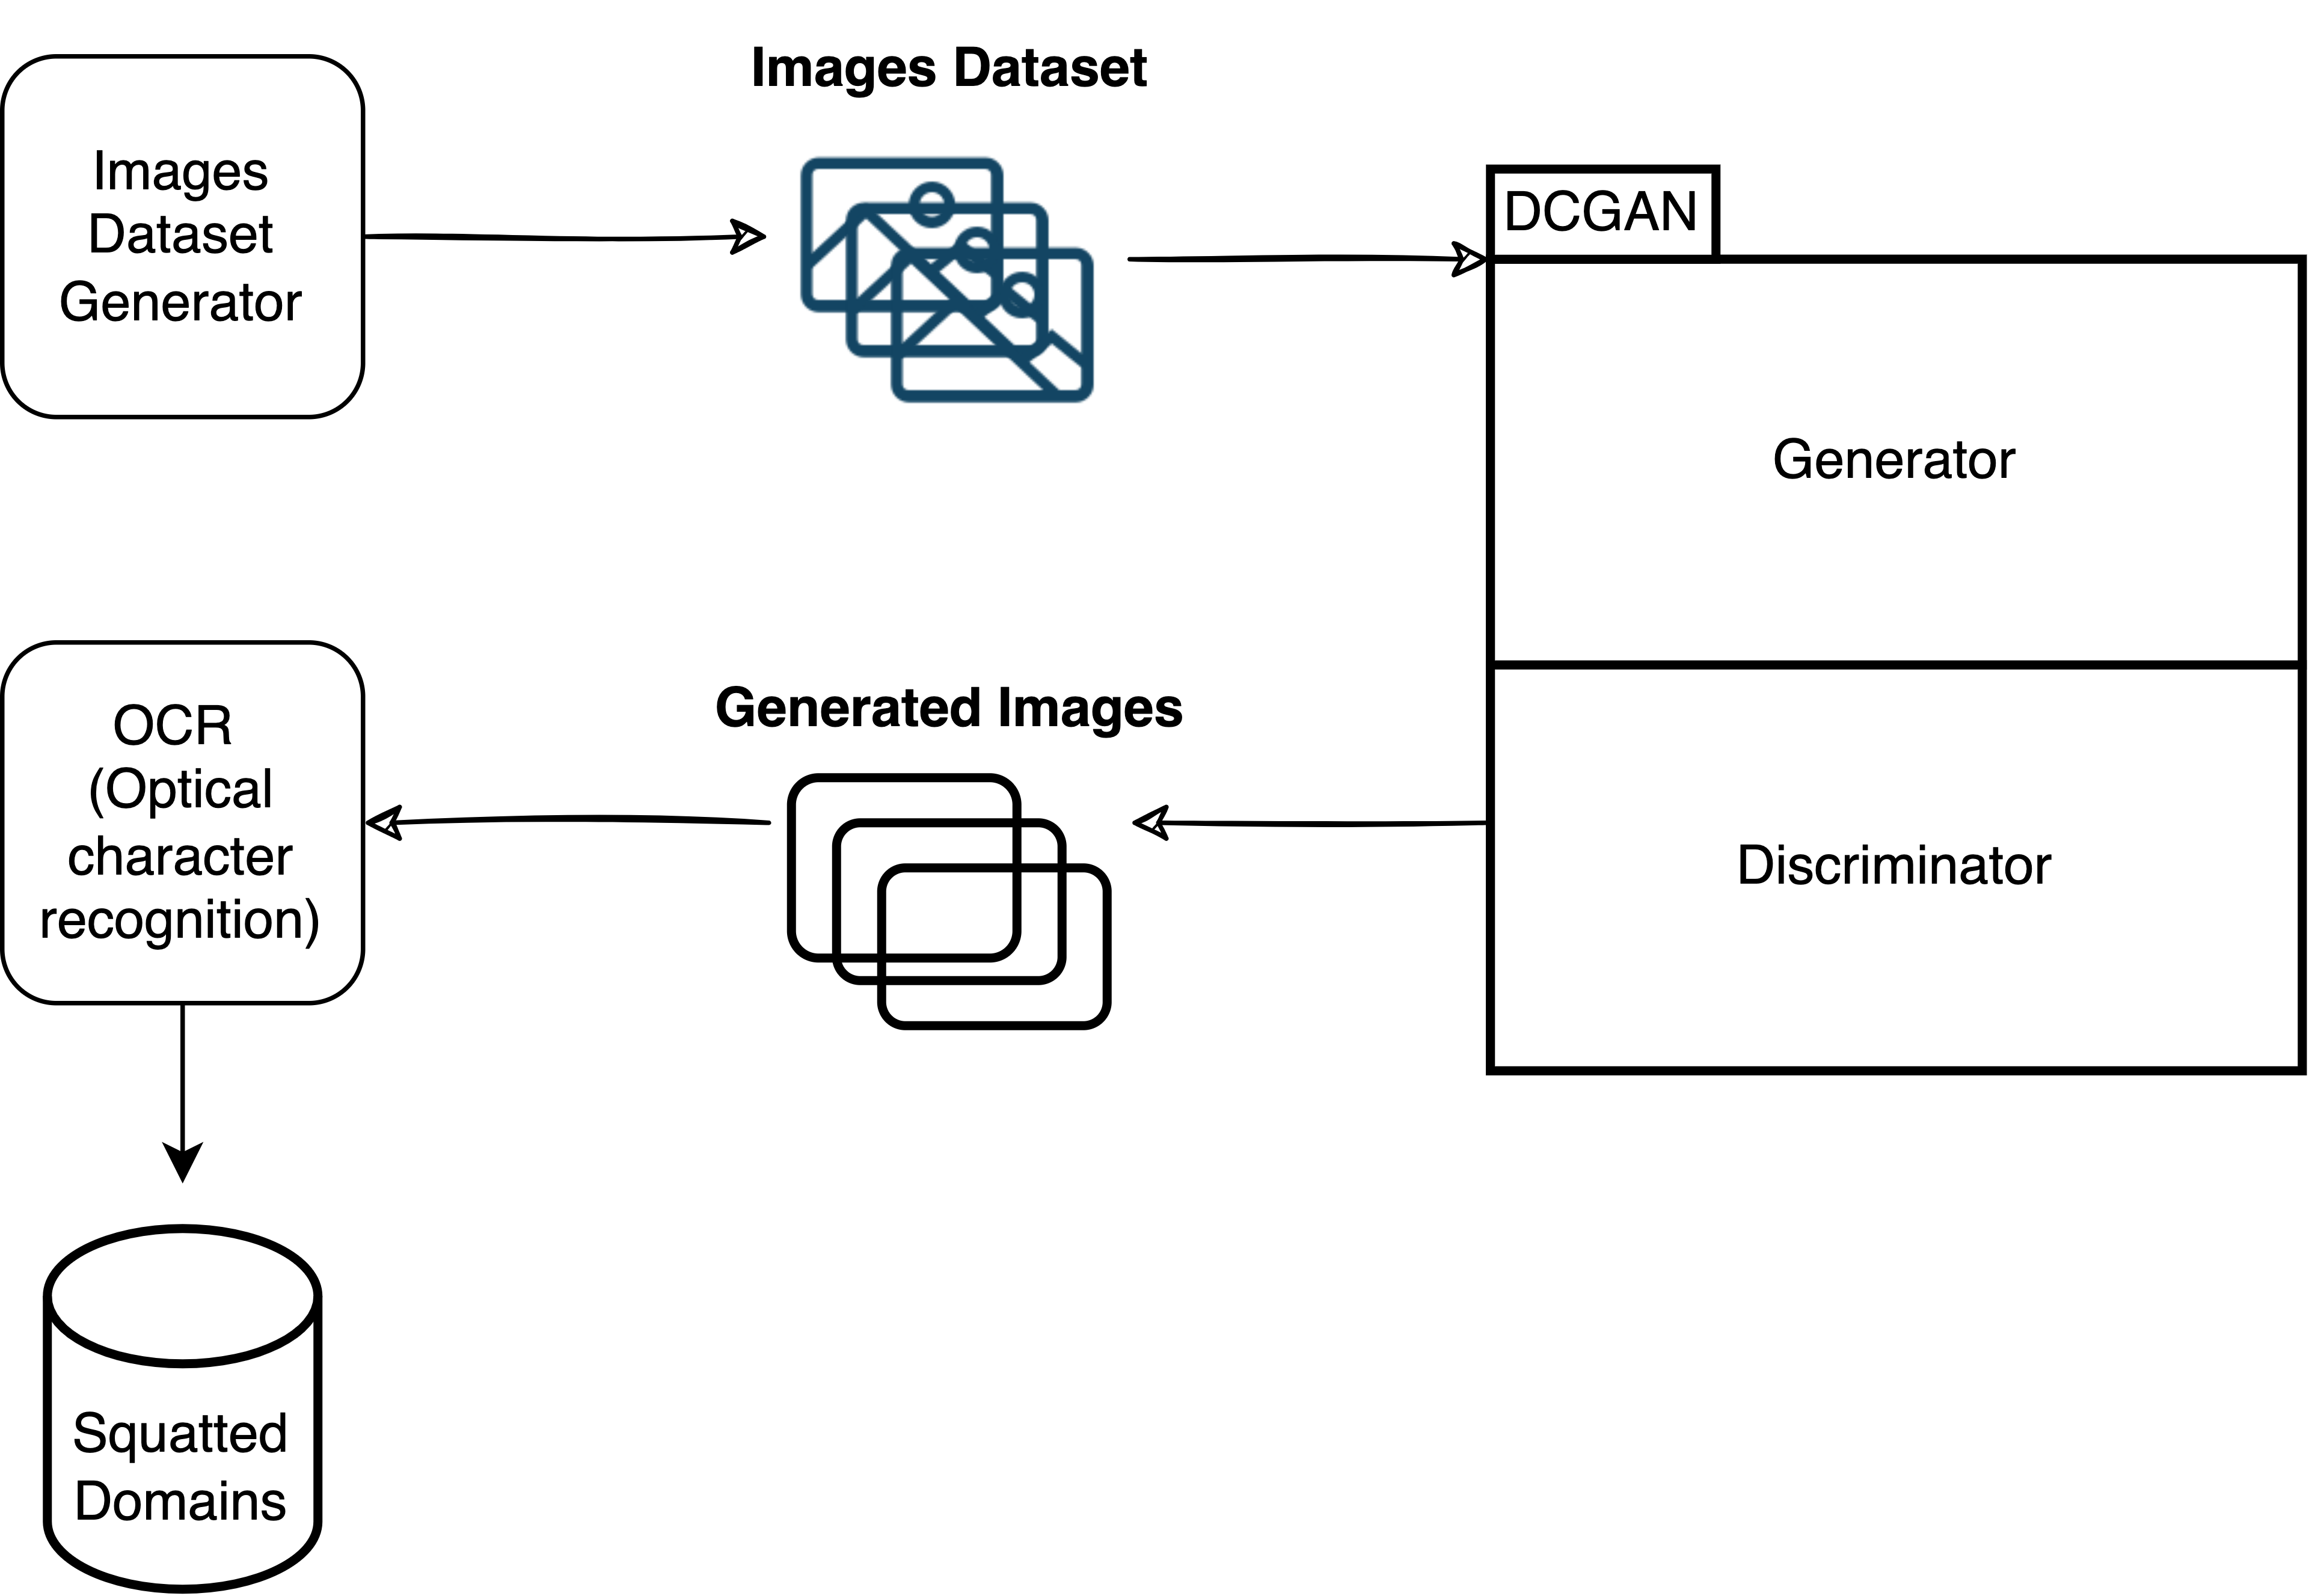
\includegraphics[width=\textwidth]{pictures/arch.png}
    \caption{SquatGAN high level architecture}
    \label{fig:arch1}
  \end{minipage}
  \hfill
\end{figure}

\section{Dataset \& training}
Per la generazione del dataset, ho fatto ricorso all'ausilio di Google Fonts per avere a disposizione una quantità di font esaustiva che mi ha permesso di testare la rete neurale anche utilizzando diversi tipi di font (ma ne parlerò più avanti).
Partendo dalla generazione del dataset di immagini, si è utilizzato la libreria PIL(Pillow) di python per produrre delle immagini partendo da del testo (che nel nostro caso il testo in input saranno nomi di dominio). Per un test preliminare ho utilizzato un singolo font per testare il comportamento della GAN su un dataset che non avesse troppa varianza sui dati, senza aggiungere rumore di alcun tipo.\\
In una versione successiva ho provato ad aggiugnere alle immagini generate (sempre attraverso l'utilizzo di PIL) del rumore all'immagine per verificare il comportamento della DCGAN e le relative immagini generate dal modello.\\
Una versione più avanzata del modello (di cui non parlerò in questo articolo) consisterebbe nel dare in pasto alla rete le immagini generate fino a quel momento.%%%%%%
\section{Modello di GAN}
Il modello di DCGAN sviluppato in una prima versione riceve come input immagini di dimensione 400 x 40 x 1 (1 canale in scala di grigio) normalizzate tra 0 e 1.
Il modello è stato costruito utilizzando principalmente in python utilizzando le librerie di Keras e Tensorflow insieme all'ausilio di altre librerie come ad esempio numpy per avere delle strutture dati efficienti su cui memorizzare i tensori.
Il generatore è descritto secondo la tabella \ref{table:generator}\\
\begin{table}[!h]
    \centering
    \begin{tabular}{|l|l|l|l|l|}
    \hline
    Filters  & Strides & Kernel & Layer           & Dropout \\ \hline
    5*50*256 & ()      & ()     & Dense           & 0.1     \\
    256      & (2, 2)  & (5, 5) & Conv2DTranspose & 0.1     \\
    128      & (2, 2)  & (5, 5) & Conv2DTranspose & 0.1     \\
    1        & (2, 2)  & (5, 5) & Conv2DTranspose & 0       \\
    \hline
    \end{tabular}
    \caption{SquatGAN generator}
    \label{table:generator}
\end{table}\\
\begin{figure}[!h]
  \centering
  \begin{minipage}[b]{\textwidth}
    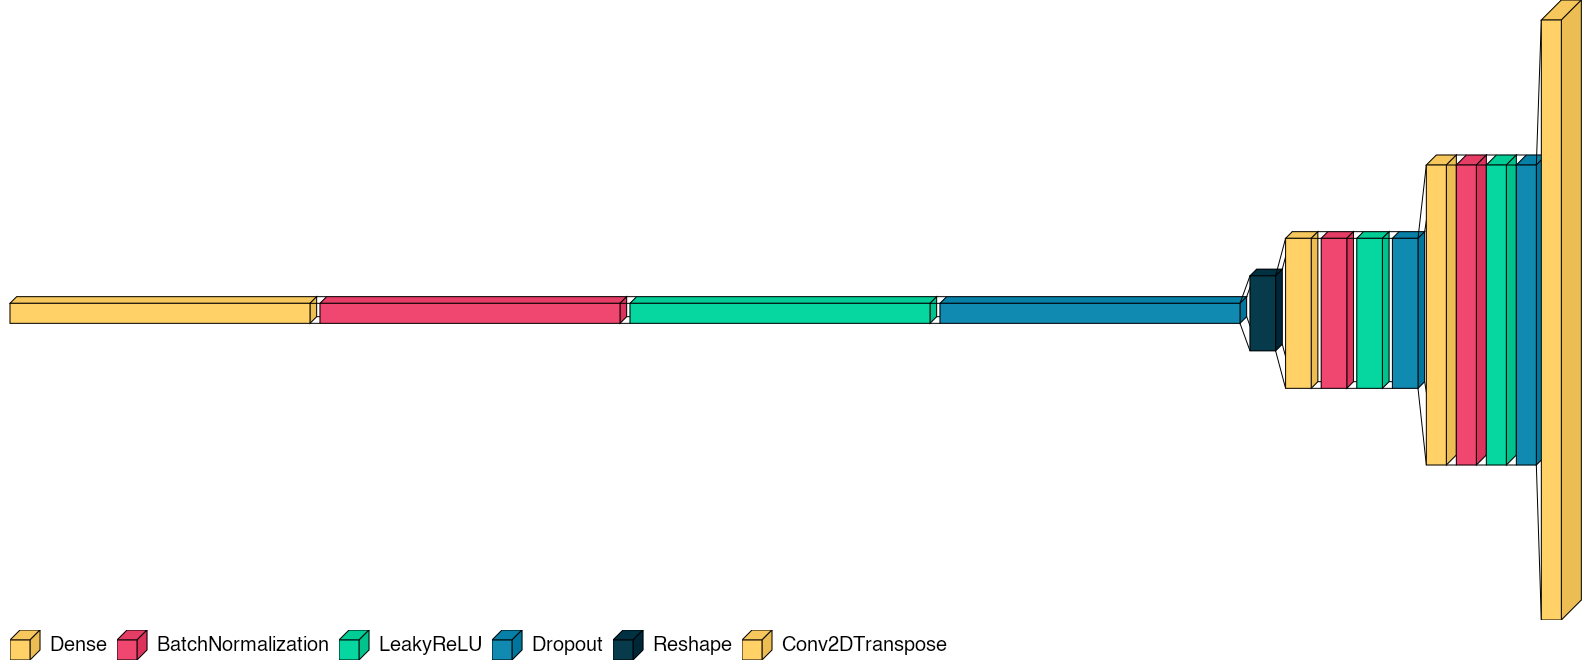
\includegraphics[width=\textwidth]{pictures/generator.png}
    \caption{SquatGAN generator}
  \end{minipage}
  \label{fig:arch}
  \hfill
\end{figure}
%%%%%%%%%%%%%%%%%%%%https://github.com/paulgavrikov/visualkeras
Ogni strato di Deconvoluzione (conv2DTranspose) è seguito da un BatchNormalization attivato da una LeakyRELU seguito da uno strato di pooling (MAX), Il batch size è stato settato a 256 per tutte le versioni. Per quanto rigurada il discriminatore, è possibile visualizzarlo attraverso la tabella \ref{table:discriminator}
\begin{table}[!h]
    \centering
    \begin{tabular}{|l|l|l|l|l|}
    \hline
    Filters & Strides & Kernel & Layer  & Dropout \\ \hline
    16      & (2, 2)  & (3, 5) & Conv2D & 0.1     \\
    32      & (2, 2)  & (3, 5) & Conv2D & 0.1     \\
    64      & (2, 2)  & (3, 5) & Conv2D & 0.1     \\
    128     & (2, 2)  & (3, 5) & Conv2D & 0.1     \\
    128     & (2, 2)  & (3, 5) & Conv2D & 0.1     \\
    256     & ()      & ()     & Dense  & 0       \\
    128     & ()      & ()     & Dense  & 0       \\
    64      & ()      & ()     & Dense  & 0       \\
    \hline
    \end{tabular}
    \caption{SquatGAN discriminator}
    \label{table:discriminator}
\end{table}


\section{Modulo OCR}
Il modulo di OCR si occupa dell'interpretazione delle immagini in testo. Nel nostro contesto, le immagini che il modulo OCR riceve sono quelle che il modello GAN produce in output dalla generazione, mentre il testo in uscita dal modulo OCR restituisce i potenziali domini squatted che sono stati generati dalle immagini della DCGAN.
Per sviluppare l'OCR ho utilizzato sempre python come linguaggio di programmazione, sfruttando Keras-OCR che permette appunto di interpretare le immagini in stringhe di testo.